\chapter{Results}

\begin{figure}[b]
	\centering
	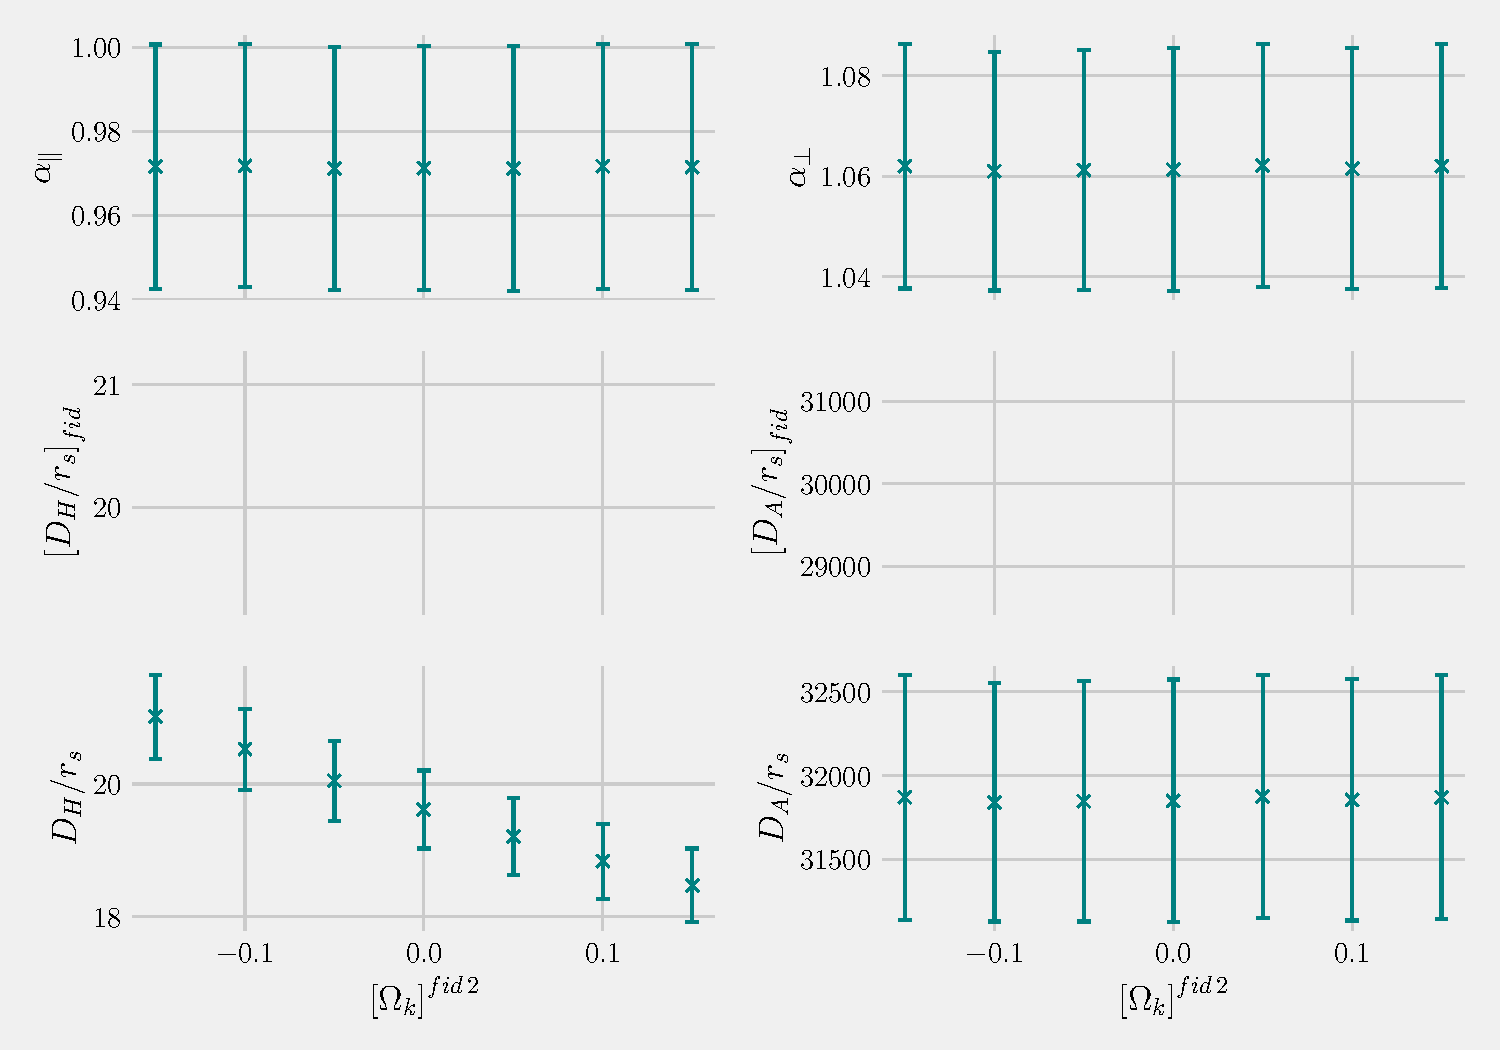
\includegraphics[width=0.99\textwidth]{../figs/phase4_DA_DH_flat.pdf}
	\caption{Calculations of the different observables $D_H /r_s$, $D_A /r_s$, both the fiducial quantities and their actual values for each fiducial curvature parameter $\Omega_k$.}
	\label{fig:DA_DH}
\end{figure}

\begin{figure}[b]
	\centering
	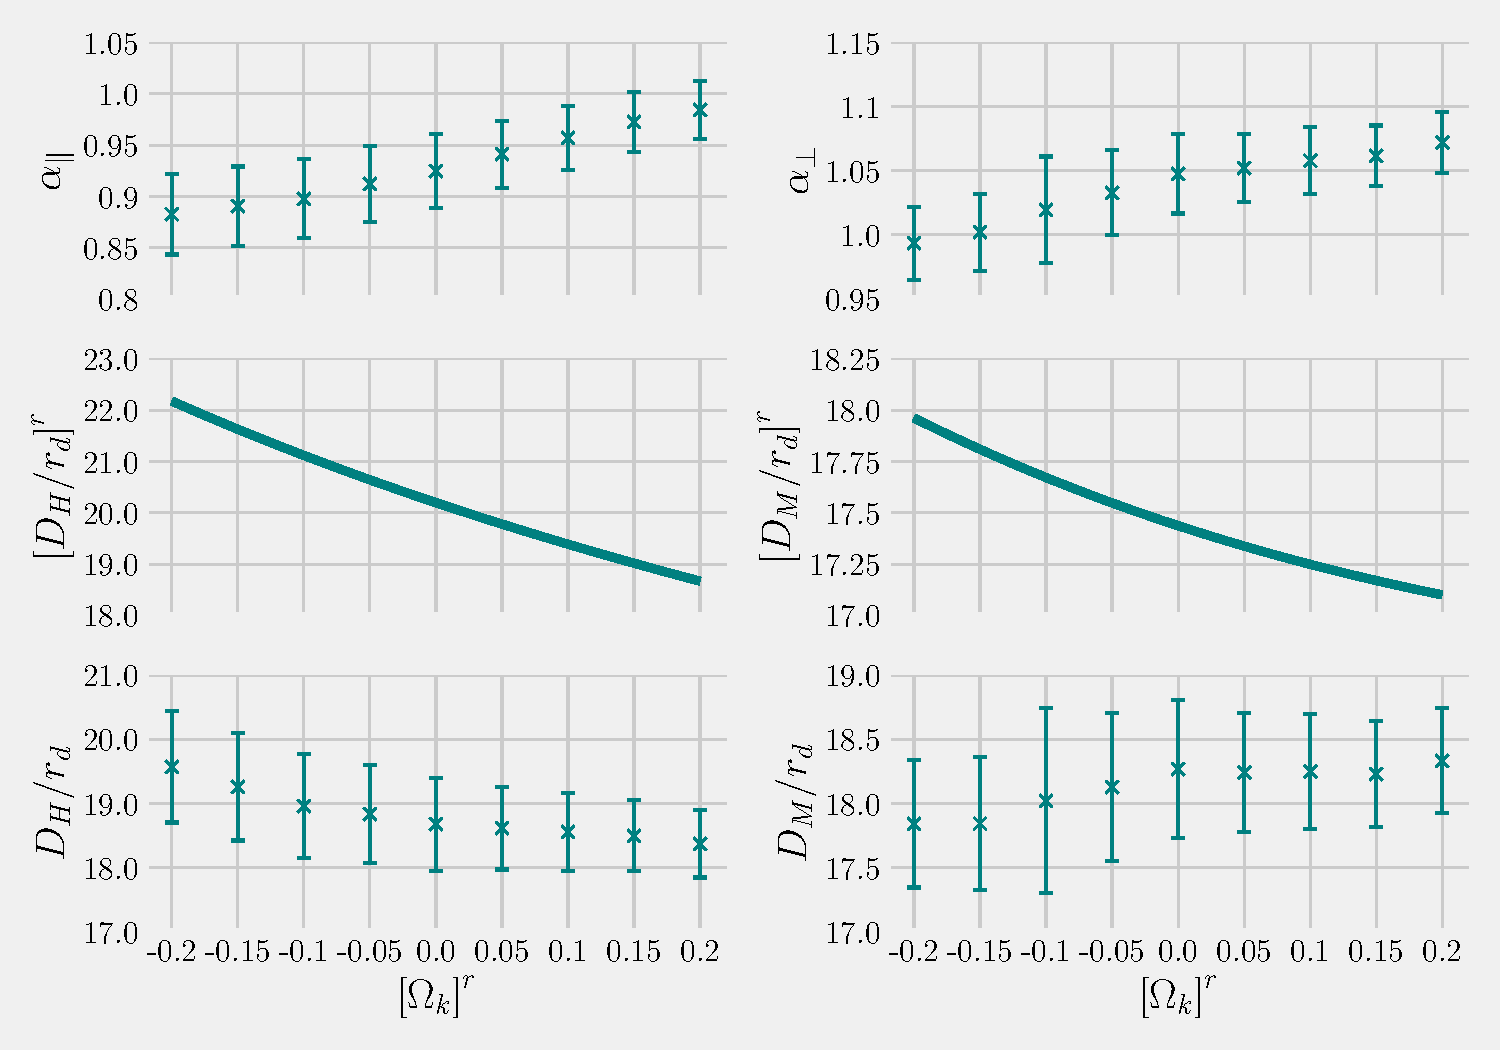
\includegraphics[width=0.99\textwidth]{../figs/phase2_DA_DH_flat.pdf}
	\caption{Calculations of the different observables $D_H /r_s$, $D_A /r_s$, both the fiducial quantities and their actual values for each fiducial curvature parameter $\Omega_k$.}
	\label{fig:DA_DH}
\end{figure}

Using the tools mentioned in the chapter~\ref{cap:met-mat}, we obtain the data seen in the figure~\ref{fig:DA_DH}. Firstly, a template power spectrum $P(k)$ was generated using CLASS. This template stays fixed throughout the calculations, which means its fiducial cosmology will be that of the standard cosmological model. This is, with the six parameters stated in~\ref{sec:LCDM} and $\Omega_k=0.00$. Having the template, the BAO are removed using the \textit{remove\_bao} routine from montepython, to obtain exactly the plots seen in~\ref{fig:PkOlPsm}.

For this fixed template, 9 different power spectrums were calculated using RUSTICO\@. We again use the $\Lambda$CDM, but this time not assuming a flat universe. Each power spectrum is generated with $\Omega_k$ from -0.20 to 0.20, in steps of 0.05, thus yielding the mentioned 9 different power spectrums.

For each one of these $\Omega_k$, the software BRASS was used to calculate each corresponding $\alpha$, and its standard deviation. This can be seen in the figure~\ref{fig:DA_DH}, which presents the $\alpha_\parallel$ and $\alpha_\perp$ on the first row, the fiducial $D_H / r_s$, $D_A/r_s $ on the second row and the `true' $D_H / r_s$, $D_A /r_s$ for each fiducial cosmology. The superscript $^{fid\, 1}$ refers to the fact that $\Omega_k$ changes only in the RUSTICO calculations. 

These observables, ($D_H /r_s$ and $D_A /r_s $) were calculated using the definitions~\eqref{eq:DH-definition} and~\eqref{eq:DA-definition}.

The BRASS calculations were done in an iterative way, which means the output from the software was used as the initial condition for the next iteration. To assure better results three iterations were made for each cosmology. 

The figure~\ref{fig:DA_DH} shows the results of the calculation of the different observables for different fiducial curvature parameters $\Omega_k$. This chart allows us to observe that the all the calculated observables in the range $\Omega_k  \in \left[ -0.20, 0.20   \right] $ are compatible, since they all stand at less than one standard deviation from one another.

